\begin{figure}[h!]
\begin{center}
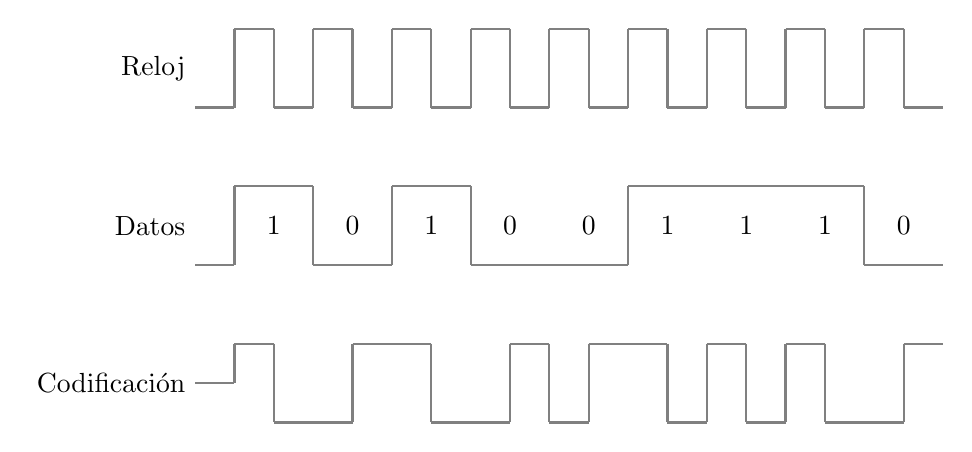
\begin{tikzpicture}
\shorthandoff{<>."}
\draw[thick,gray] (0,2) -- (0.5,2);
\draw[thick,gray] (0.5,2) -- (0.5,3);
\draw[thick,gray] (0.5,3) -- (1,3);
\draw[thick,gray] (1,3) -- (1,2);
\draw[thick,gray] (1,2) -- (1.5,2);
\draw[thick,gray] (1.5,2) -- (1.5,3);
\draw[thick,gray] (1.5,3) -- (2,3);
\draw[thick,gray] (2,3) -- (2,2);
\draw[thick,gray] (2,2) -- (2.5,2);
\draw[thick,gray] (2.5,2) -- (2.5,3);
\draw[thick,gray] (2.5,3) -- (3,3);
\draw[thick,gray] (3,3) -- (3,2);
\draw[thick,gray] (3,2) -- (3.5,2);
\draw[thick,gray] (3.5,2) -- (3.5,3);
\draw[thick,gray] (3.5,3) -- (4,3);
\draw[thick,gray] (4,3) -- (4,2);
\draw[thick,gray] (4,2) -- (4.5,2);
\draw[thick,gray] (4.5,2) -- (4.5,3);
\draw[thick,gray] (4.5,3) -- (5,3);
\draw[thick,gray] (5,3) -- (5,2);
\draw[thick,gray] (5,2) -- (5.5,2);
\draw[thick,gray] (5.5,2) -- (5.5,3);
\draw[thick,gray] (5.5,3) -- (6,3);
\draw[thick,gray] (6,3) -- (6,2);
\draw[thick,gray] (6,2) -- (6.5,2);
\draw[thick,gray] (6.5,2) -- (6.5,3);
\draw[thick,gray] (6.5,3) -- (7,3);
\draw[thick,gray] (7,3) -- (7,2);
\draw[thick,gray] (7,2) -- (7.5,2);
\draw[thick,gray] (7.5,2) -- (7.5,3);
\draw[thick,gray] (7.5,3) -- (8,3);
\draw[thick,gray] (8,3) -- (8,2);
\draw[thick,gray] (8,2) -- (8.5,2);
\draw[thick,gray] (8.5,2) -- (8.5,3);
\draw[thick,gray] (8.5,3) -- (9,3);
\draw[thick,gray] (9,3) -- (9,2);
\draw[thick,gray] (9,2) -- (9.5,2);

\node[left] at (0,2.5){Reloj};

\draw[thick,gray] (0,0) -- (0.5,0);
\draw[thick,gray] (0.5,0) -- (0.5,1);
\draw[thick,gray] (0.5,1) -- (1.5,1);
\draw[thick,gray] (1.5,1) -- (1.5,0);
\draw[thick,gray] (1.5,0) -- (2.5,0);
\draw[thick,gray] (2.5,0) -- (2.5,1);
\draw[thick,gray] (2.5,1) -- (3.5,1);
\draw[thick,gray] (3.5,1) -- (3.5,0);
\draw[thick,gray] (3.5,0) -- (5.5,0);
\draw[thick,gray] (5.5,0) -- (5.5,1);
\draw[thick,gray] (5.5,1) -- (8.5,1);
\draw[thick,gray] (8.5,1) -- (8.5,0);
\draw[thick,gray] (8.5,0) -- (9.5,0);

\node[left] at (0,0.5){Datos};
\node at (1,.5){1};
\node at (2,.5){0};
\node at (3,.5){1};
\node at (4,.5){0};
\node at (5,.5){0};
\node at (6,.5){1};
\node at (7,.5){1};
\node at (8,.5){1};
\node at (9,.5){0};

\draw[thick,gray] (0,-1.5) -- (0.5,-1.5);
\draw[thick,gray] (0.5,-1.5) -- (0.5,-1);
\draw[thick,gray] (0.5,-1) -- (1,-1);
\draw[thick,gray] (1,-1) -- (1,-2);
\draw[thick,gray] (1,-2) -- (2,-2);
\draw[thick,gray] (2,-2) -- (2,-1);
\draw[thick,gray] (2,-1) -- (3,-1);
\draw[thick,gray] (3,-1) -- (3,-2);
\draw[thick,gray] (3,-2) -- (4,-2);
\draw[thick,gray] (4,-2) -- (4,-1);
\draw[thick,gray] (4,-1) -- (4.5,-1);
\draw[thick,gray] (4.5,-1) -- (4.5,-2);
\draw[thick,gray] (4.5,-2) -- (5,-2);
\draw[thick,gray] (5,-2) -- (5,-1);
\draw[thick,gray] (5,-1) -- (6,-1);
\draw[thick,gray] (6,-1) -- (6,-2);
\draw[thick,gray] (6,-2) -- (6.5,-2);
\draw[thick,gray] (6.5,-2) -- (6.5,-1);
\draw[thick,gray] (6.5,-1) -- (7,-1);
\draw[thick,gray] (7,-1) -- (7,-2);
\draw[thick,gray] (7,-2) -- (7.5,-2);
\draw[thick,gray] (7.5,-2) -- (7.5,-1);
\draw[thick,gray] (7.5,-1) -- (8,-1);
\draw[thick,gray] (8,-1) -- (8,-2);
\draw[thick,gray] (8,-2) -- (9,-2);
\draw[thick,gray] (9,-2) -- (9,-1);
\draw[thick,gray] (9,-1) -- (9.5,-1);

\node[left] at (0,-1.5){Codificaci\'on};

\shorthandon{<>."}
\end{tikzpicture}
\end{center}
\caption[Proceso de codificaci\'on]{Proceso de codificaci\'on de una se\~nal transformada a datos.}
\label{fig:cod}
\end{figure}